\scanpage{67}
passage aux complémentaires) les dix ``triangles'' de $I$, correspondent aux dix faces de l'icosaèdre gauche ($\simeq$ paires de faces opposées de l'icos. ordinaire), tandis que les $15$ partitions de type $(2,2,1)$ de $I$, qu'on peut interpréter comme les structures carrées sur quatre parmi les $5$ pts de $I$
\figure{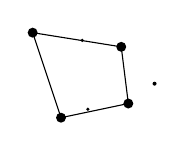
\begin{tikzpicture}[scale=.9]\draw (0,1.1)--(1.25,.9)--(1.35,.1)--(.4,-.1)--cycle;\foreach \p in {(0,1.1),(1.25,.9),(1.35,.1),(.4,-.1)}{\fill \p circle (2pt);}\fill (.7,.99) circle (.7pt);\fill (.78,.02) circle (.7pt);\fill (1.72,.38) circle (.8pt);\end{tikzpicture}}
(en associant à un tel carré les deux paires de sommets diagonalement opposés) correspondent aux $15$ arêtes dudit icosaèdre gauche.
\margin{NB on associe à un côté $a$ le jeu des ``couleurs'' des $4$ autres côtés des faces adjacentes, groupées \deleted{\unsure{deux}} en deux paires \unsure{des deux faces}.
\figure{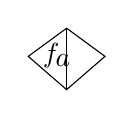
\begin{tikzpicture}[scale=.65]\draw (0,0)--(.75,.55)--(1.5,0)--(.75,-.65)--cycle;\draw (.75,.55)--(.75,-.65);\node at (.45,.02) {$f$};\node at (.68,-.08) {$a$};\end{tikzpicture}}}
Un côté \inserted{$a$} est contenu \deleted{dans}\inserted{(incident)} à une face \inserted{$f$} de l'icosaèdre, sss le ``triangle'' $\subset I$ correspondant à $f$ a comme intersection avec le carré correspondant à $a$, \deleted{deux}\inserted{l'un des} \deleted{\unsure{côt}} $2$ sommets \deleted{consécutifs}\inserted{opposés} du carré, \deleted{On voit donc.}\inserted{i.e. ssi le complémentaire du triangle est formé de l'une des deux paires définissant le carré.}
\inserted{Donc on voit que} la relation d'incidence des diviseurs à \unsure{sommets} de la structure $\widehat M_{0,I}$, correspond à celle des faces et arêtes de l'icosaèdre gauche, ou par dualité, à celle des \deleted{arêtes}\inserted{sommets} et des \deleted{faces}\inserted{arêtes} du dodécaèdre.

On a donc trouvé :
\margin{66}
